\documentclass[a4paper]{article}
\usepackage[T1]{fontenc} % Polskie znaki
\usepackage{graphicx} % Wstwianie grafiki
\usepackage{subcaption}
\usepackage{float}
%opening
\title{Rozpoznawanie stanu rozgrywki w grze planszowej Catan}
\author{Magdalena Wiechczyńska, 132337\\
Piotr Tomaszewski, 136821}
\date{} %Usunięcie daty

\begin{document}

\maketitle

\section{Temat i opis rozwiązania problemu}
	Program na podstawie zdjęcia planszy gry Catan rozpoznaje stan rozgrywki, tzn. ułożenie heksagonalnych pól reprezentujących surowce oraz rozstawienie pionków graczy (gracza czerwonego, niebieskiego i pomarańczowego).
	
	W pierwszym kroku stara się wyizolować na zdjęciu samą planszę, aby pominąć w przetwarzaniu elementy nie należące do gry. Następnie po kolei lokalizowane są kolejne typy pól, zaczynając od
tych najbardziej wyróżniających się. Pola znajdywane są na podstawie selekcji pikseli należących
do zadanego przedziału wartości HSV. W celu ułatwienia poszukiwania kolejnych, już znalezione pola
na bieżąco są usuwane ze zdjęcia poddawanego przetwarzaniu. W przypadku identyfikacji niektórych pól zbliżonych kolorystycznie koniecznym jest skalowanie saturacji zdjęcia, dodatkowo zastosowano również filtr medianowy.

	Pionki graczy znajdywane są analogicznie. Miasta i osady są odróżniane od dróg na podstawie podobieństwa kształtu do koła (miasta mają okrągłą podstawę, osady natomiast, pomimo nieregularnego kształtu, stanowią dość dobre przybliżenie koła).

	
\section{Działanie programu}
    \subsection{Znajdowanie planszy}
     Na początku program próbuje ustalić położenie planszy i usunąć wszelkie elementy do niej nienależące.

    Wiedząc, że plansza do gry jest zawsze otoczona ramką przedstawiającą wodę, wyszukujemy pikseli, których wartość odcienia (Hue) w przestrzeni HSV należy do odpowiedniego przedziału. Następnie, w celu usunięcia dziur uzyskany obraz poddajemy dylatacji.
    \begin{figure}[H]
        \centering
        \begin{subfigure}[t]{.3\linewidth}
        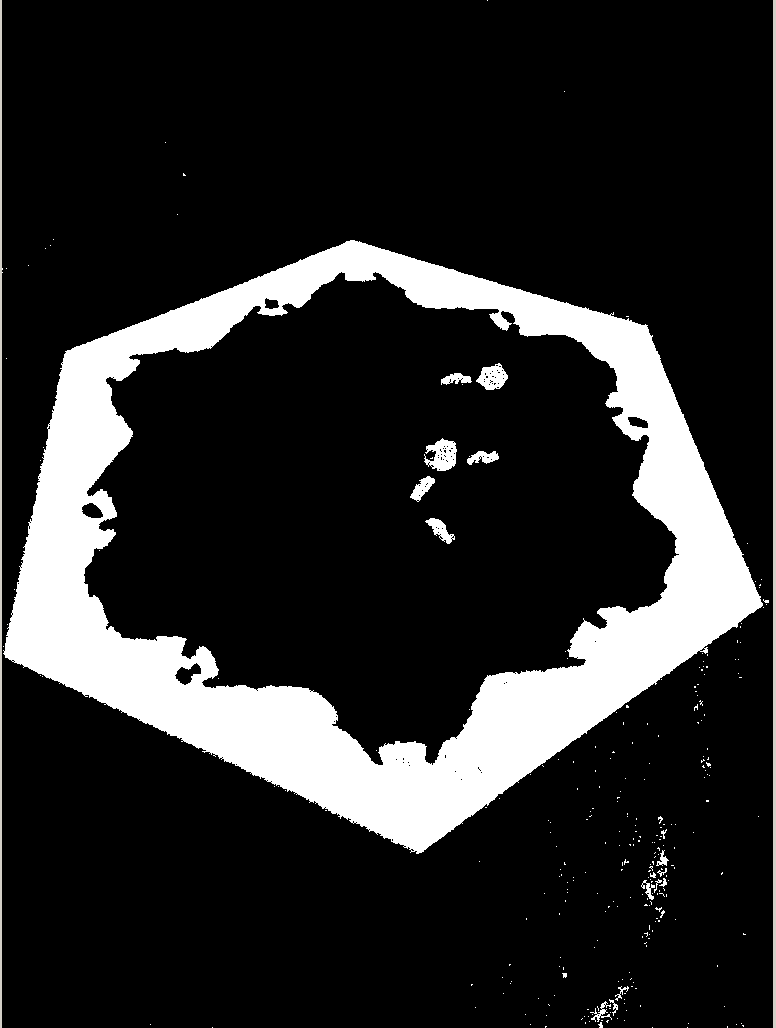
\includegraphics[width=\linewidth]{pictures/steps/find_water.png}
        \subcaption{Wycięta ramka}
        \end{subfigure}
        \begin{subfigure}[t]{.3\linewidth}
        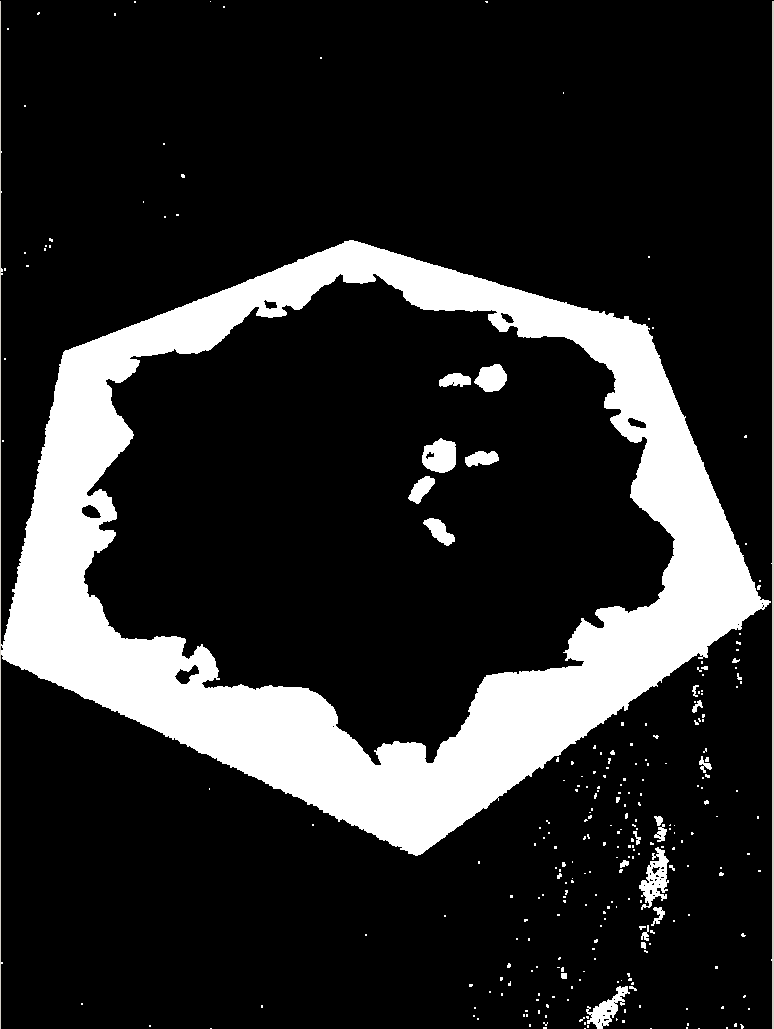
\includegraphics[width=\linewidth]{pictures/steps/find_water_dilate.png}
        \subcaption{Wycięta ramka poddana dylatacji}
        \end{subfigure}

        \caption{Znajdowanie ramki}
        \label{fig:step1a}
    \end{figure}

    Na tak przetworzonym obrazie szukamy konturów. Zależy nam na znalezieniu wewnętrznego konturu planszy. Na większości zdjęć jest to drugi kontur pod względem obejmowanego pola powierzchni. Jednak, w przypadku gdy ramka zdjęcia jest prześwietlona, oba konutury łączą się w jeden. Dlatego w celu ustalenia, który kontur jest konturem wewnętrznym sprawdzamy czy na danym zdjęciu drugi pod względem wielkości kontur znajduje się wewnątrz największego.

    Następnie zastępujemy kolorem czarnym wszystkie piksele, które nie znajdują się wewnątrz tego konturu.
    \begin{figure}[H]
        \begin{subfigure}[t]{0.3\linewidth}
            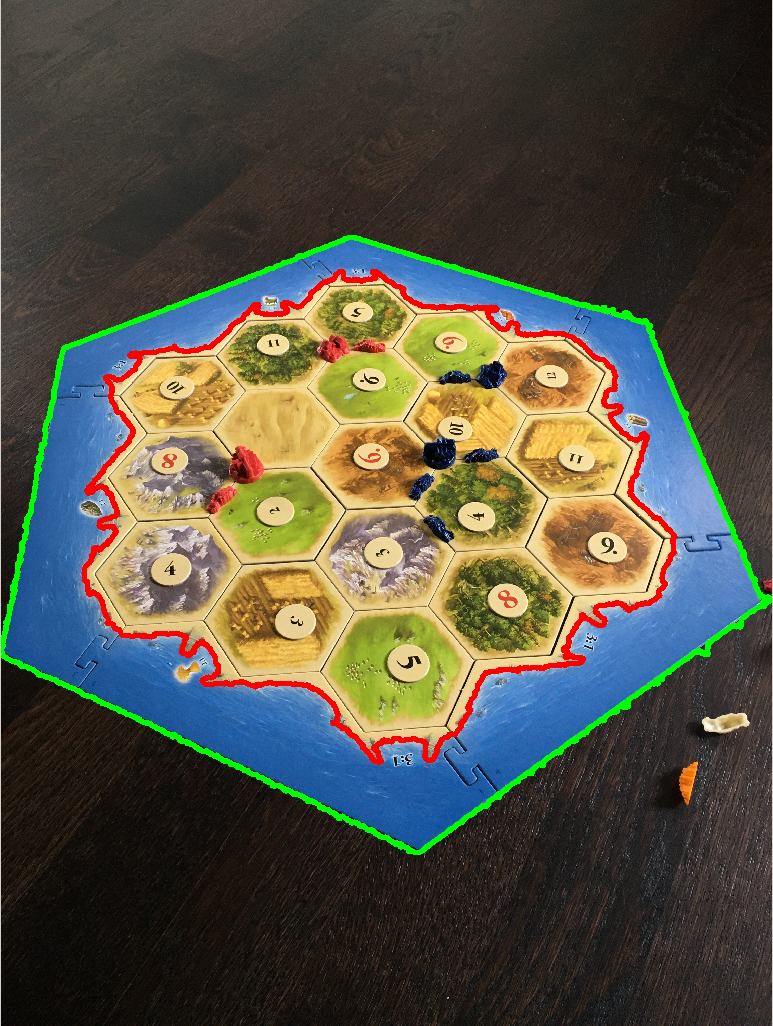
\includegraphics[width=\linewidth]{pictures/steps/two_contours.png}
            \subcaption{Dwa największe kontury}
        \end{subfigure}
        \begin{subfigure}[t]{0.3\linewidth}
            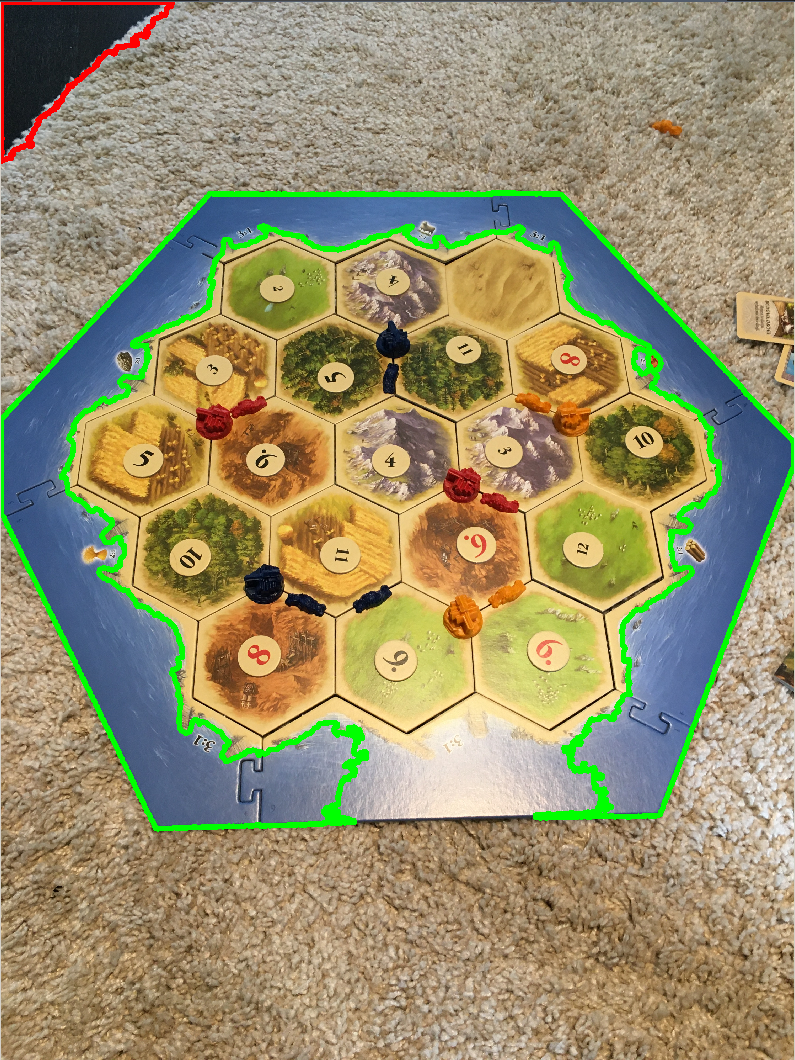
\includegraphics[width=\linewidth]{pictures/steps/two_contours_blend.png}
            \subcaption{Kontury łączą się ze sobą}
        \end{subfigure}
        \begin{subfigure}[t]{0.3\linewidth}
            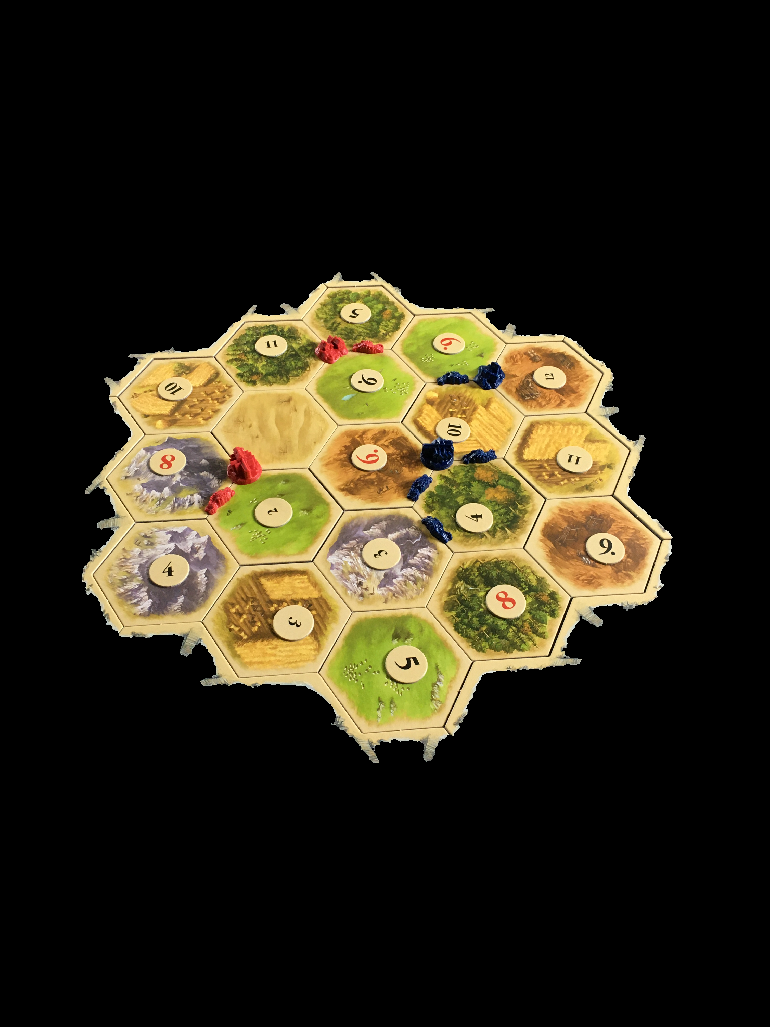
\includegraphics[width=\linewidth]{pictures/steps/background_cut.png}
            \subcaption{Wycięte tło}
        \end{subfigure}
        \caption{Wycinanie tła}
        \label{fig:step1b}
    \end{figure}

    \subsection{Znajdowanie pionków}
       Poszukiwanie pionków odbywa się dla każdego koloru (czerwonego, niebieskiego i pomarańczowego) z osobna.
    Za każdym razem poszukujemy pikseli, które należą do określonego obszaru przestrzeni barw HSV.
    Przykładowo, dla pionków koloru niebieskiego przedziały znormalizowanych wartości H, S i V prezentują się następująco:
    H = [0.58, 0.69], S = [0.3, 1], V = [0, 0.6].
    Uzyskana w ten sposób maska zostaje następnie, w zależności od koloru, poddana erozji/dylatacji.
     \begin{figure}[H]
        \begin{subfigure}[t]{0.3\linewidth}
            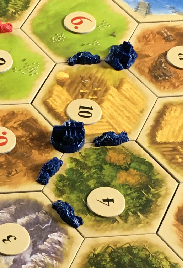
\includegraphics[width=\linewidth]{pictures/steps/pawns_fragment.png}
            \subcaption{Fragment obrazu}
        \end{subfigure}
%
        \begin{subfigure}[t]{0.3\linewidth}
            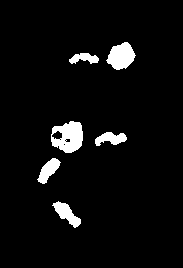
\includegraphics[width=\linewidth]{pictures/steps/pawns_mask.png}
            \subcaption{Uzyskana maska}
        \end{subfigure}
%
        \begin{subfigure}[t]{0.3\linewidth}
            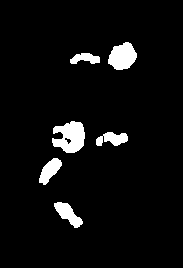
\includegraphics[width=\linewidth]{pictures/steps/pawns_mask_dilated.png}
            \subcaption{Maska poddana dylatacji}
        \end{subfigure}
        \caption{Znajdowanie pionków na obrazie}
    \end{figure}

    \subsection{Rozpoznawanie pionków}
    Na każdej masce, uzyskanej w poprzednim kroku, szukamy konturów. Dla każdego z nich wyznaczamy otoczkę wypukłą (convex hull), ponieważ pionki wykonane są z błyszczącego plastiku i trudno jest zapewnić, aby w całości były zaznaczone na masce.

    Następnie w każdą otoczkę, której powierzchnia znajduje się w akceptowalnym przedziale wpasowywana jest elipsa.
    Liczymy stosunek półosi wielkiej do półosi małej elipsy. Dla miast i osad stosunek ten jest bliski 1, natomiast drogi są bardziej podłużne, więc dla nich ten stosunek jest niższy.

    Jeżeli jednak powierzchnia otoczki danego konturu przekracza akceptowalną wartość, może to oznaczać, że na tym obszarze znajdują się w rzeczywistości dwa pionki. Dlatego ten kontur rysujemy na nowej, czystej masce. Maskę następnie poddajemy erozji i rekurencyjnie wywołujemy na niej funkcję rozpoznającą pionki. Robimy tak do czasu, aż powierzchnia otoczki znajdzie się w akceptowalnym przedziale.

    Dla każdego zidentyfikowanego pionka wyznaczany jest centroid, który następnie zaznaczany jest na obrazie.

    \subsection{Znajdowanie i rozpoznawanie pól}
    W pierwszej kolejności stosujemy filtr medianowy z maską 15x15. Sprawi to, że kolory zostaną wygładzone i staną się mniej różnorodne w obrębie poszczególnych pól.
    
    \begin{figure}[H]
        \begin{subfigure}[]{.5\linewidth}
        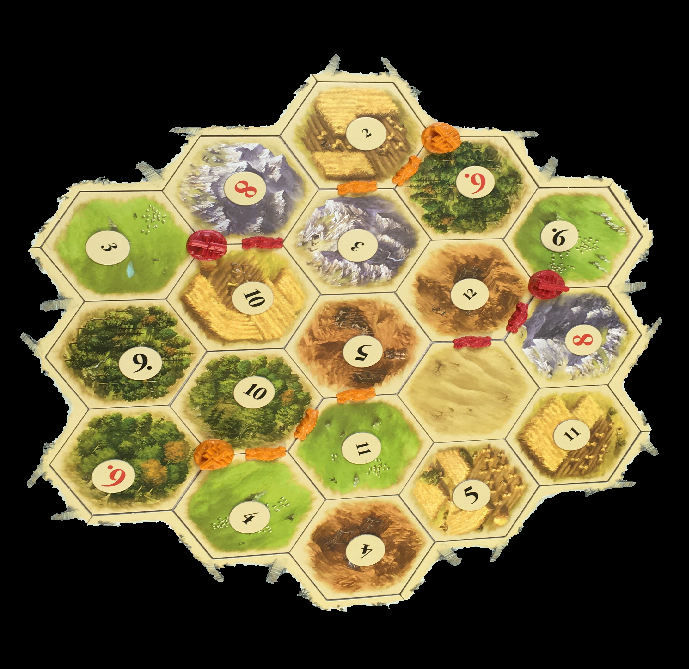
\includegraphics[width=\linewidth]{pictures/fields/pre_blur.png}
        \subcaption{Plansza przed nałożeniem filtru}

        \end{subfigure}
        \begin{subfigure}[]{0.5\linewidth}
        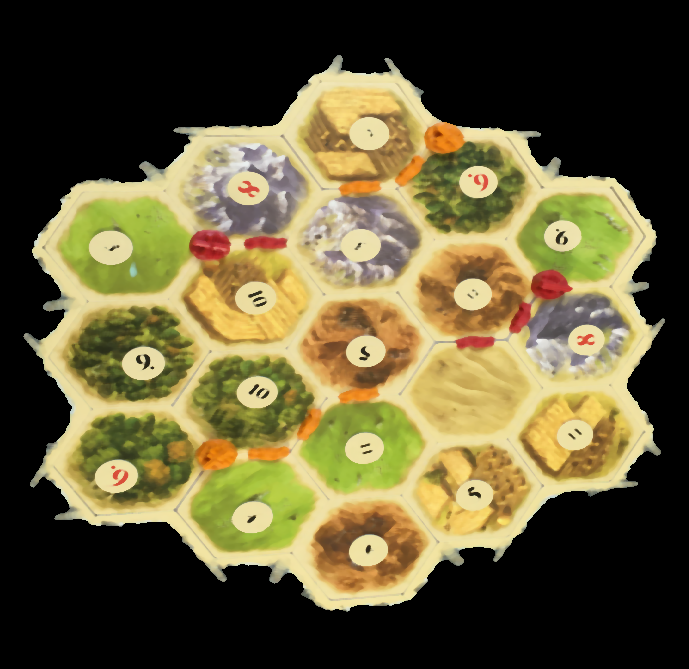
\includegraphics[width=\linewidth]{pictures/fields/after_blur.png}
        \subcaption{Plansza po nałożeniu filtru}
        \end{subfigure}

        \caption{Filtr medianowy}
        \label{fig:step3}
    \end{figure}
    
    Następnie odszukujemy najbardziej wyróżniający się typ pola, łąkę z owcami. Dokonujemy selekcji pikseli na podstawie ich wartości H, S i V (sprawdzamy czy wszystkie wartości znajdują się w akceptowalnych przedziałach. 
    
    Przykładowo, oto przedziały znormalizowanych wartości H, S, V, które lokalizują pola z owcami:
    
H = [0.15, 0.3], S = [0.4, 1], V = [0.6, 1] 
	
	\begin{figure}[H]
		
        \begin{subfigure}[]{.5\linewidth}
        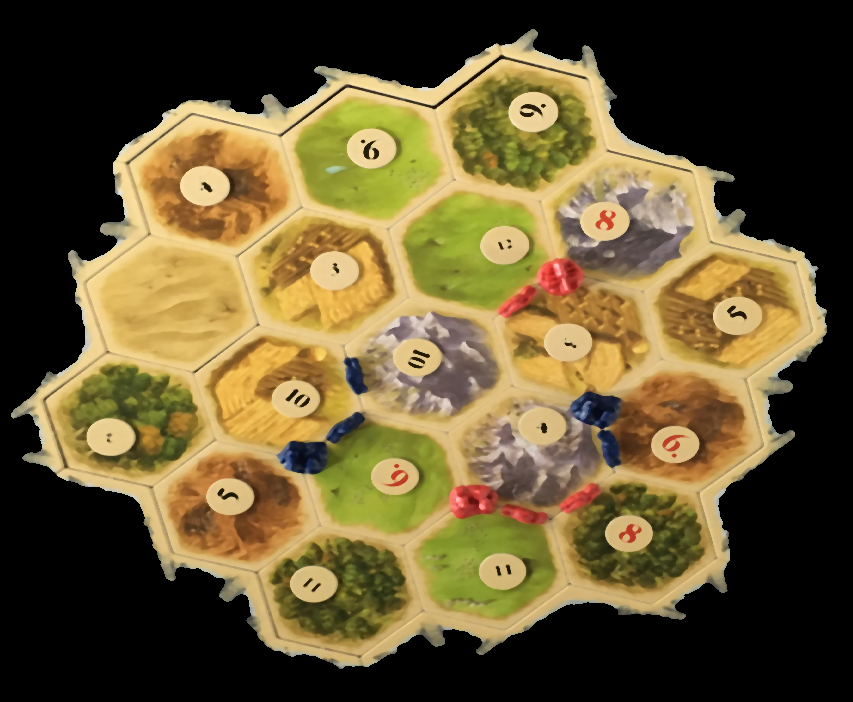
\includegraphics[width=\linewidth]{pictures/fields/pre_mask.png}
        \subcaption{Przetwarzane zdjęcie}
        \end{subfigure}
       %
        \begin{subfigure}[]{0.5\linewidth}
        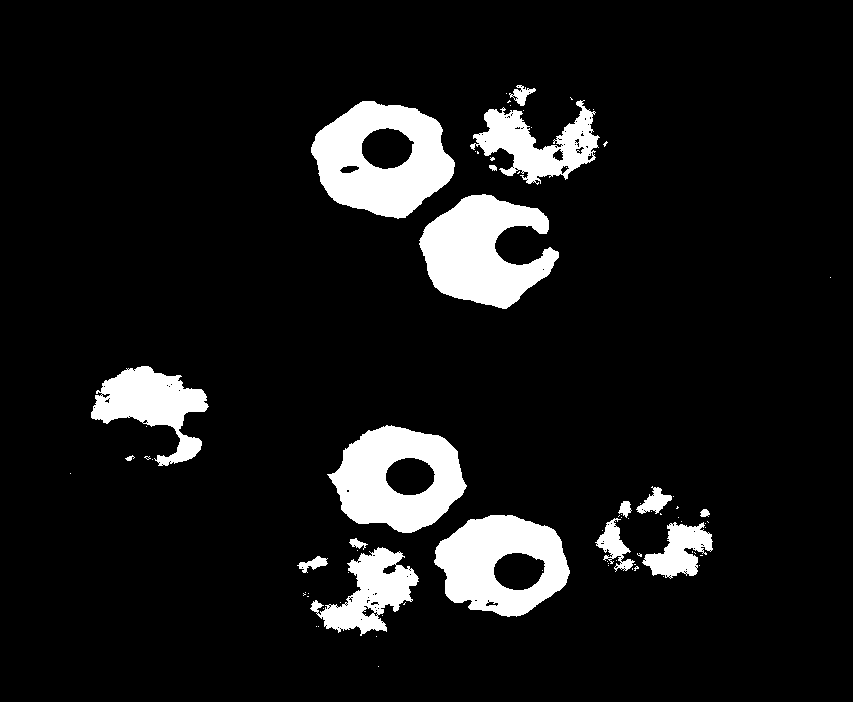
\includegraphics[width=\linewidth]{pictures/fields/after_mask.png}
        \subcaption{Wynik selekcji pikseli}
        \end{subfigure}
		\begin{subfigure}[]{0.5\linewidth}
        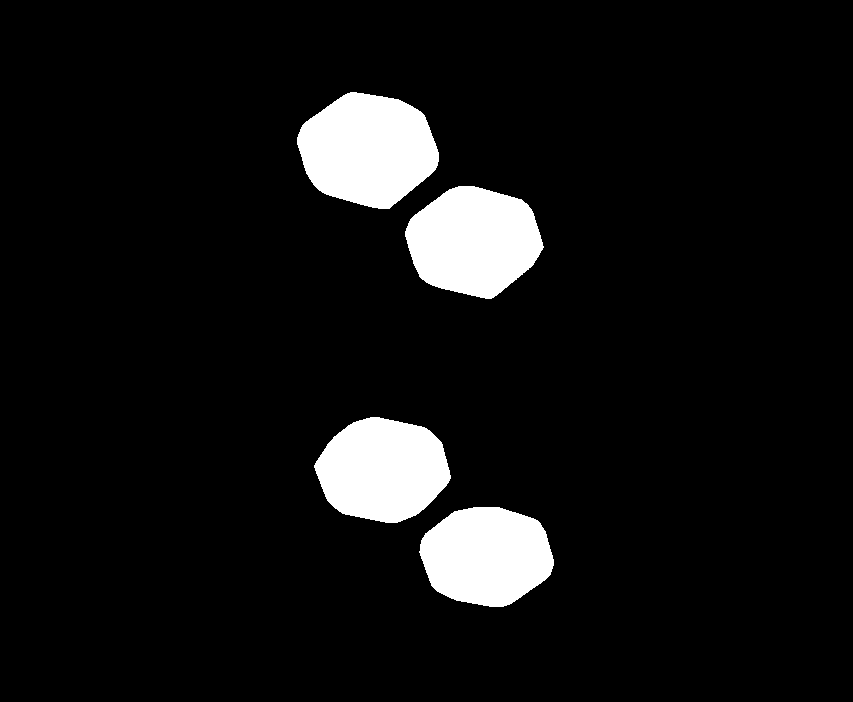
\includegraphics[width=\linewidth]{pictures/fields/convex.png}
        \subcaption{Otoczka wypukła (convex hull)}
        \end{subfigure}
        %
        \begin{subfigure}[]{0.5\linewidth}
        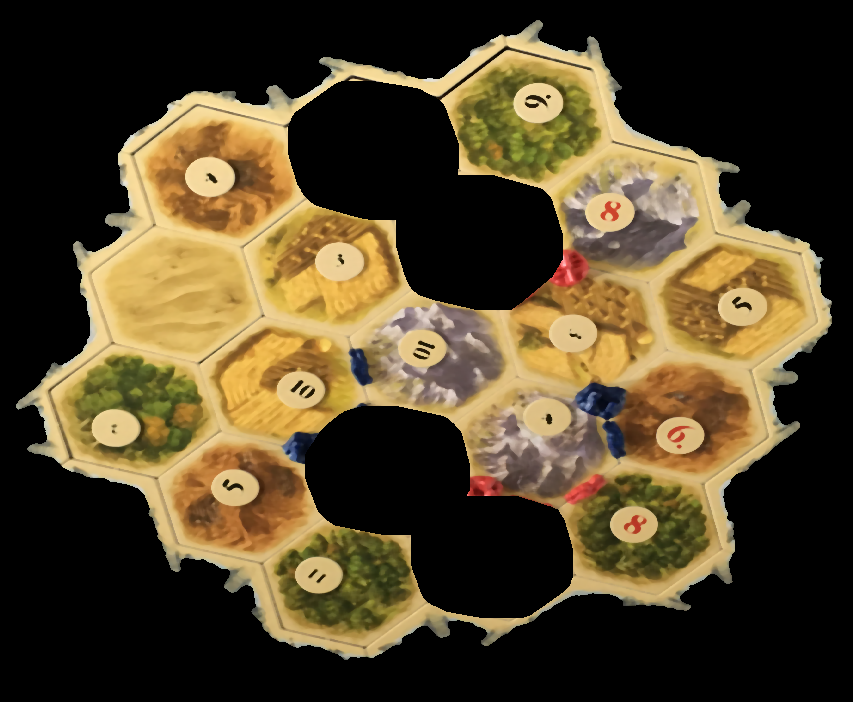
\includegraphics[width=\linewidth]{pictures/fields/delete_convex.png}
        \subcaption{Zdjęcie z wyciętymi polami}
        \end{subfigure}
        \caption{ Selekcja pikseli na podstawie akceptowalnych przedziałów wartości.}
        \label{fig:step4}
    \end{figure}
	
	Następnie, w zależności od aktualnie rozważanego typu pola, maska poddawana zostaje dylatacji/erozji. Na masce odszukujemy kontury, które następnie sortowane są pod względem pola powierzchni.
	
Wykorzystujemy fakt, że liczba poszczególnych typów pól na planszy jest stała (są zawsze cztery łąki, trzy pola z górami itd.). Z tego powodu rozważamy jedynie x pierwszych konturów z posortowanej listy.
Dla każdego z tych konturów znajdowana jest otoczka wypukła (convex hull). Na jej podstawie obliczany jest centroid i wyrysowywana jest kropka reprezentująca dane pole. 

Dodatkowo, otoczki umieszczane są na nowej masce, która jest następnie poddawana dylatacji. Tak utworzona maska wycina z przetwarzanego obrazu pola, które zostały już odnalezione. Ma to ułatwić odnajdywanie następnych typów pól.
	
Po odnalezieniu łąk w sposób analogiczny lokalizowane są lasy. Przed wyszukiwaniem gór staramy się dodatkowo wyciąć obramowanie pól, aby zminimalizować możliwość odnalezienia konturów w tych miejscach (ze względu na swoją jasność).

	\begin{figure}[H]
        \begin{subfigure}[]{.5\linewidth}
        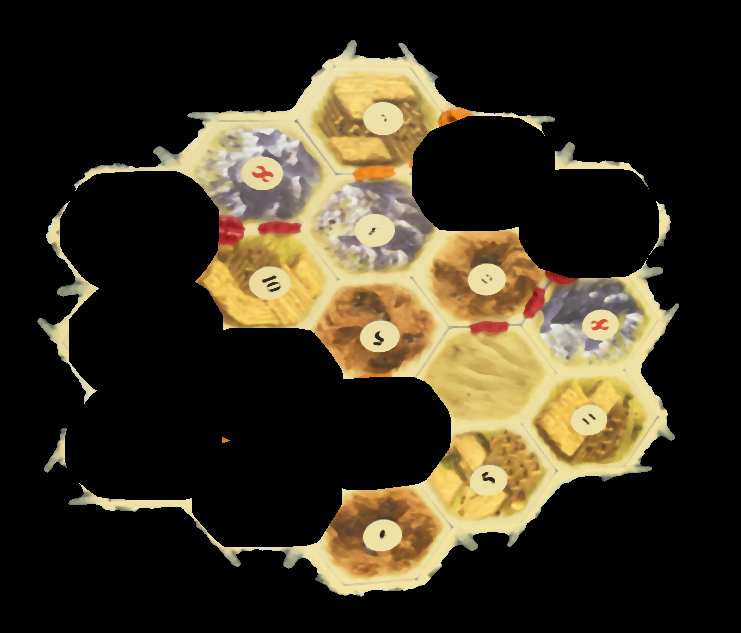
\includegraphics[width=\linewidth]{pictures/fields/pre_cut.png}
        \subcaption{Zdjęcie po usunięciu lasów}

        \end{subfigure}
        \begin{subfigure}[]{0.5\linewidth}
        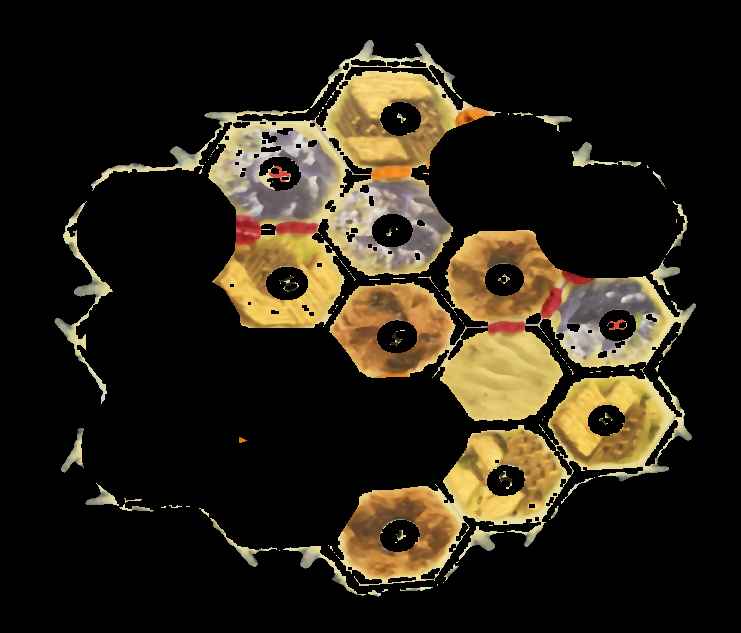
\includegraphics[width=\linewidth]{pictures/fields/after_cut.png}
        \subcaption{Odcięte obramowanie}
        \end{subfigure}

        \caption{Odcięcie obramowania planszy}
        \label{fig:step5}
    \end{figure}
	
Ostatnie pola do identyfikacji są zdecydowanie trudniejsze, ze względu na podobieństwo kolorystyczne, jednak po zastosowaniu 5-krotnego skalowania saturacji obrazu glina wystarczająco wyróżnia się na tle pozostałych pól, aby móc z powodzeniem wykorzystać wyżej przedstawiony algorytm.

	\begin{figure}[H]
        \begin{subfigure}[]{.5\linewidth}
        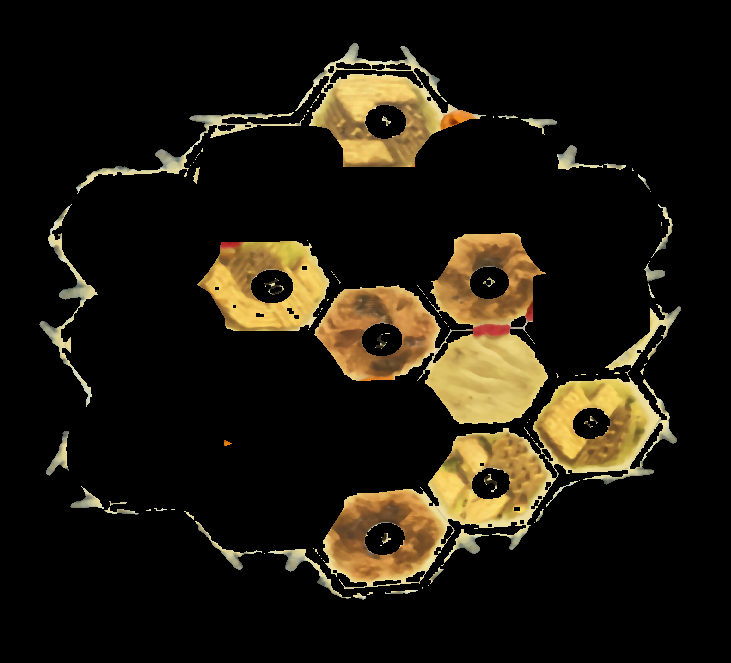
\includegraphics[width=\linewidth]{pictures/fields/pre_sat.png}
        \subcaption{Przed}

        \end{subfigure}
        \begin{subfigure}[]{0.5\linewidth}
        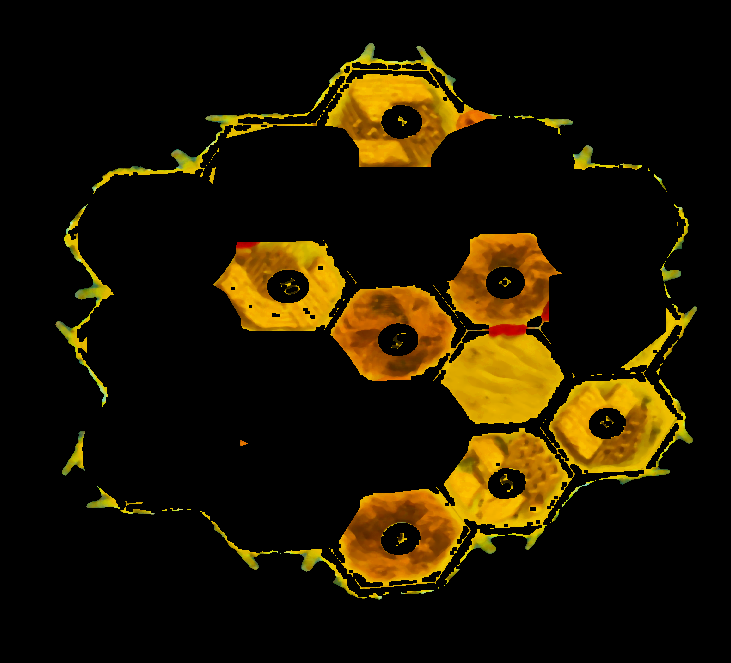
\includegraphics[width=\linewidth]{pictures/fields/after_sat.png}
        \subcaption{Po}
        \end{subfigure}

        \caption{Skalowanie saturacji, odszukanie gliny staje się łatwiejsze}
        \label{fig:step6}
    \end{figure}
	
Odróżnienie pustyni od łąk jedynie na podstawie koloru nie jest wystarczającym rozwiązaniem - delikatna różnica w oświetleniu pól może zaważyć o wyniku działania programu. W tym celu wykorzystywany jest fakt, że na pustyni nigdy nie znajdzie się okrągły krążek z liczbą, z racji tego, że pustynia reprezentuje brak surowca. Z tego powodu za jednym razem znajdujemy wszystkie pięć pozostałych w grze pól (cztery pola ze zbożem i pustynia) oraz uznajemy za pustynię ten kontur, dla którego pole powierzchni jest największe.
      
\section{Przedstawienie wyników}
    \subsection{Zdjęcia łatwe}
    
     \begin{figure}[H]
        \begin{subfigure}[]{\linewidth}
            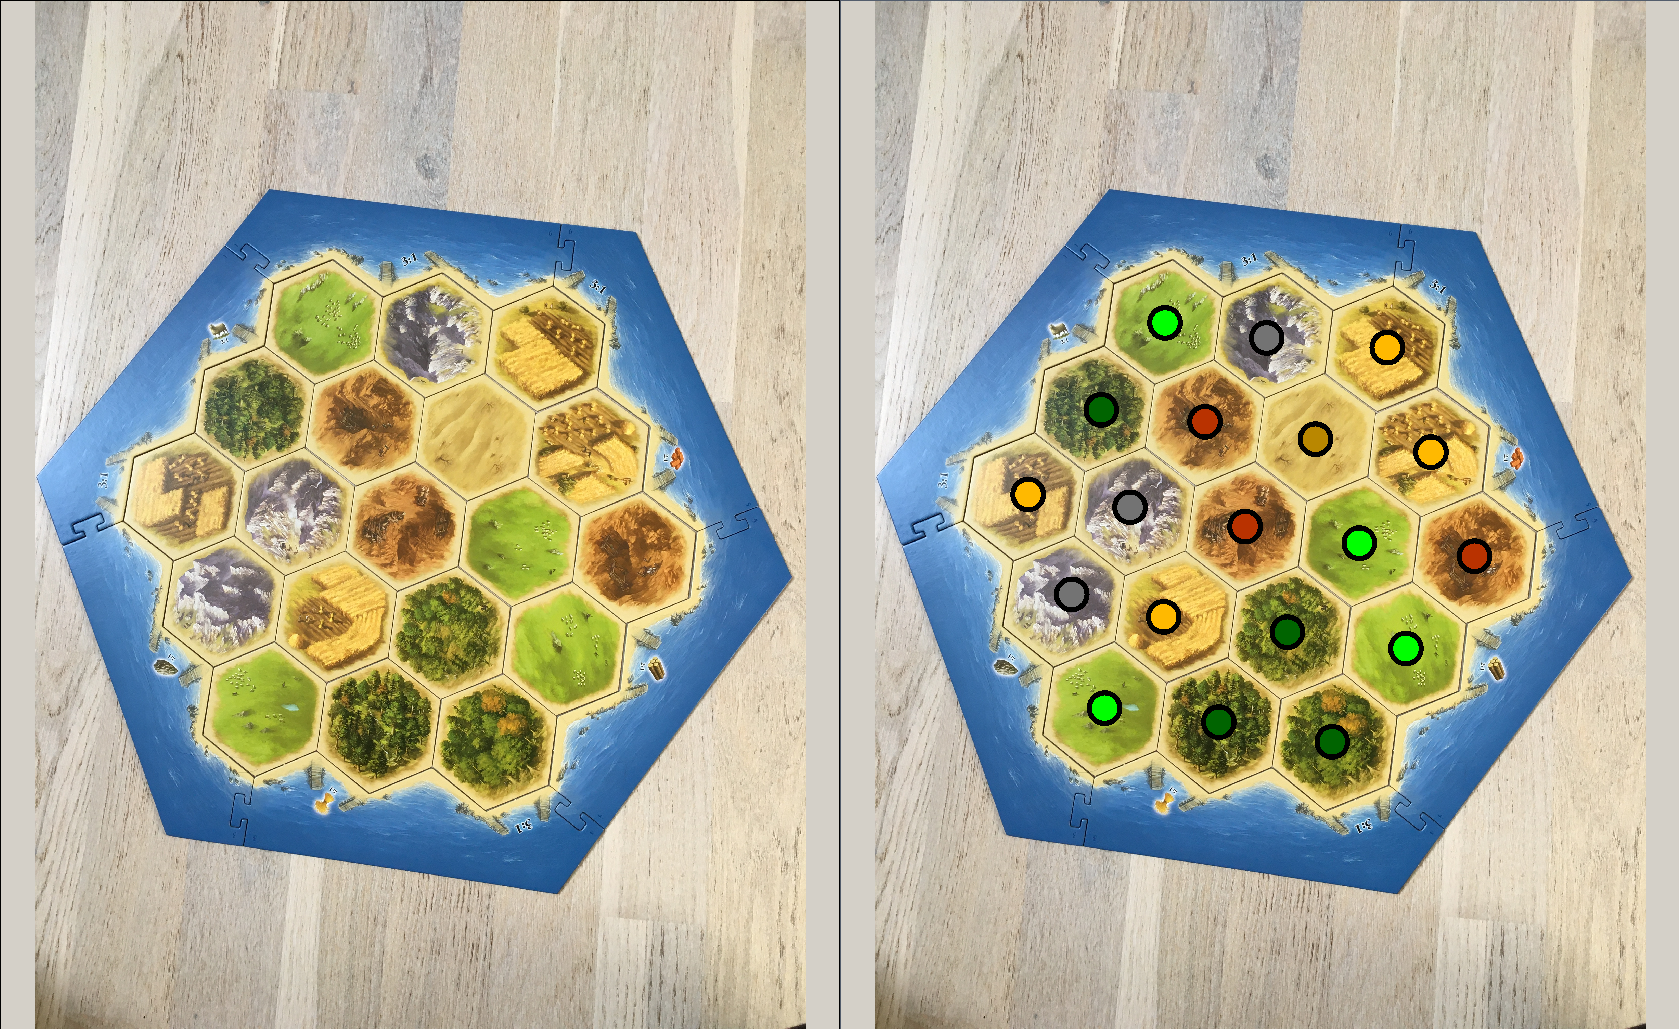
\includegraphics[width=\linewidth]{pictures/easy1.png}
            \subcaption{Brak pionków i liczb}
        \end{subfigure}

        \begin{subfigure}[]{\linewidth}
            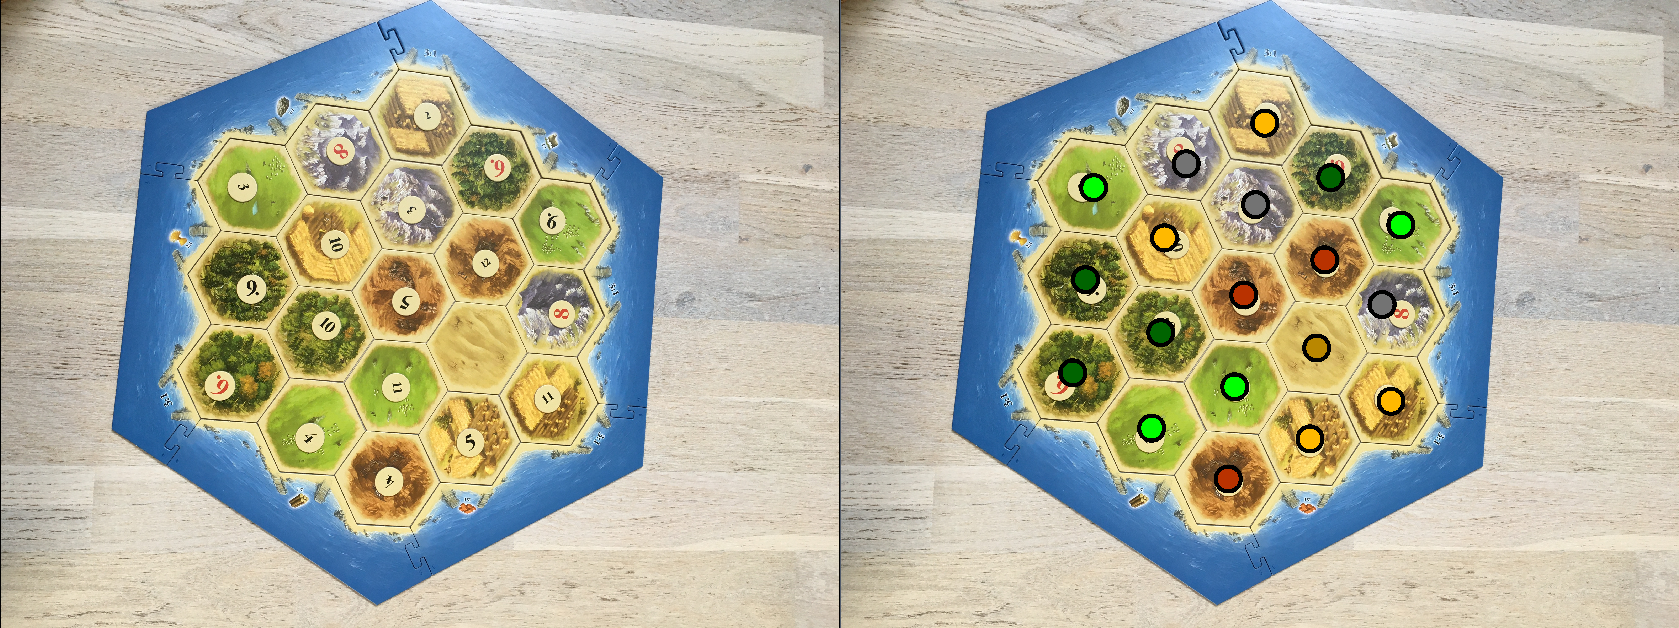
\includegraphics[width=\linewidth]{pictures/easy2.png}
            \subcaption{Liczby na planszy (brak pionków graczy)}
        \end{subfigure}
        
        \begin{subfigure}[]{\linewidth}
            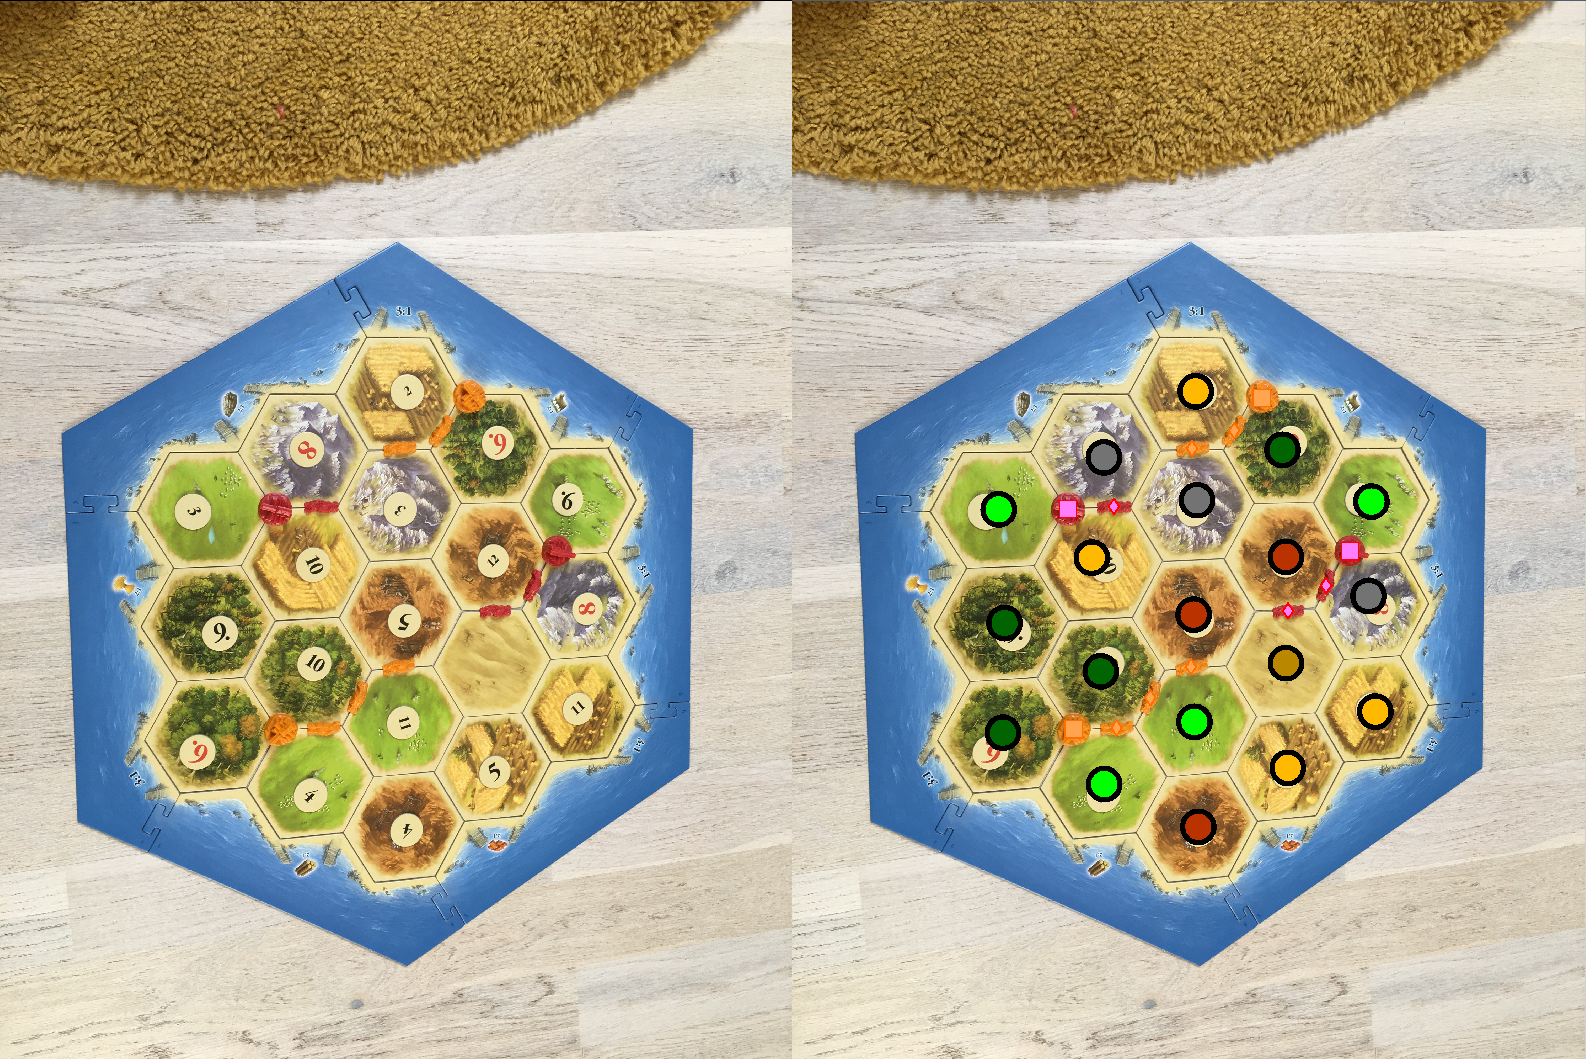
\includegraphics[width=\linewidth]{pictures/results/result04.png}
            \subcaption{Kąt prostopadły, bardzo dobre oświetlenie}
        \end{subfigure}
        
        
        \caption{Przykłady zdjęć łatwych}
        \label{fig:easy}
    \end{figure}
    
    \subsection{Zdjęcia średnie}
    
    \begin{figure}[H]
        \begin{subfigure}[]{\linewidth}
            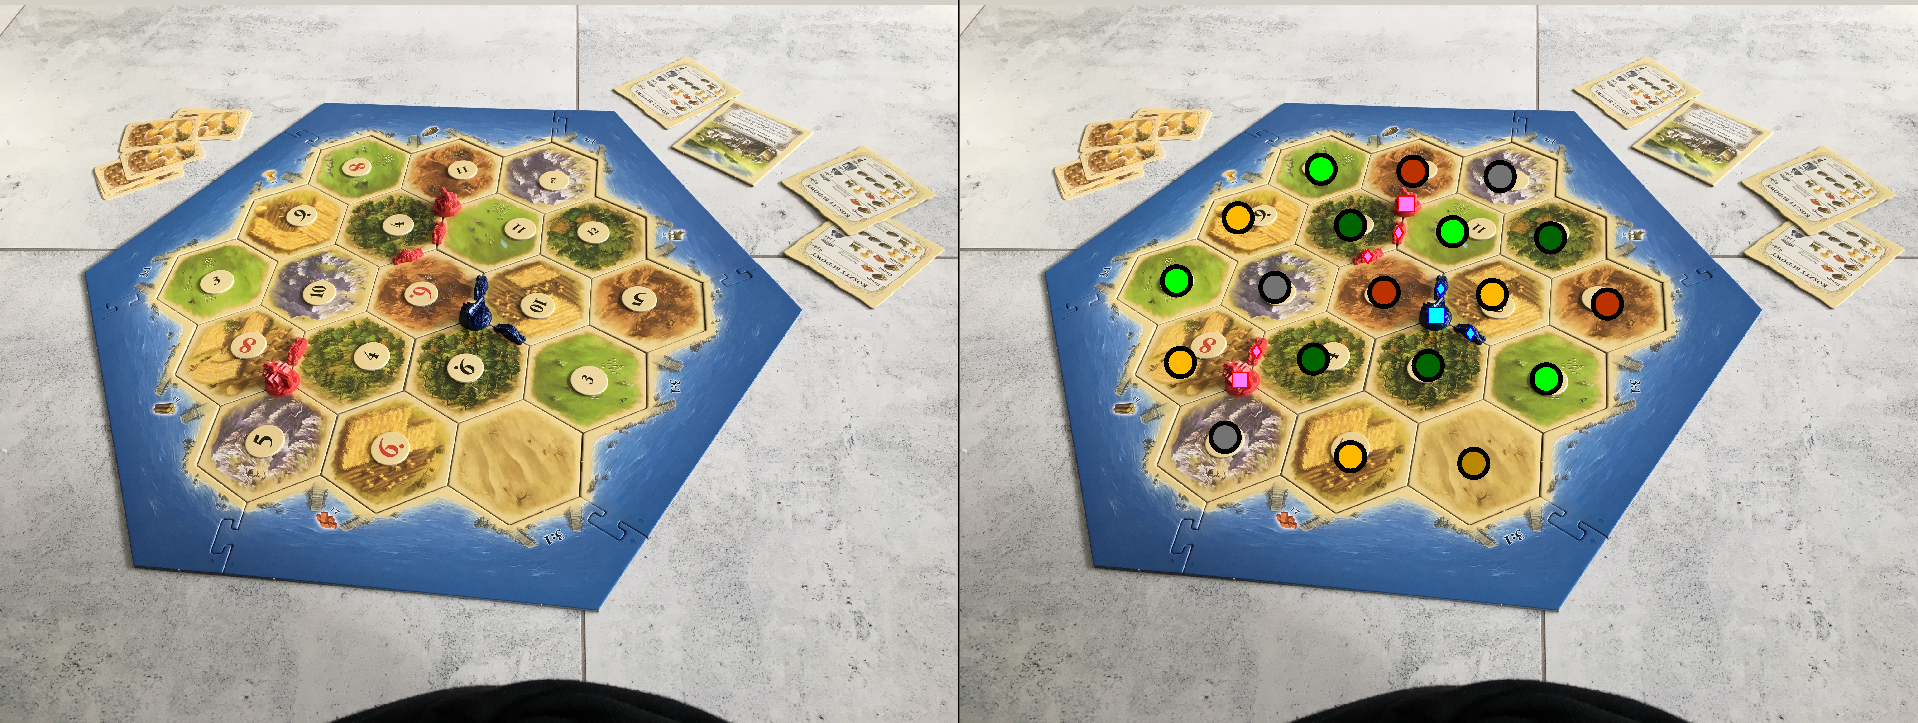
\includegraphics[width=\linewidth]{pictures/results/result19.png}
            \subcaption{Zdjęcie pod kątem}
        \end{subfigure}

        \begin{subfigure}[]{\linewidth}
            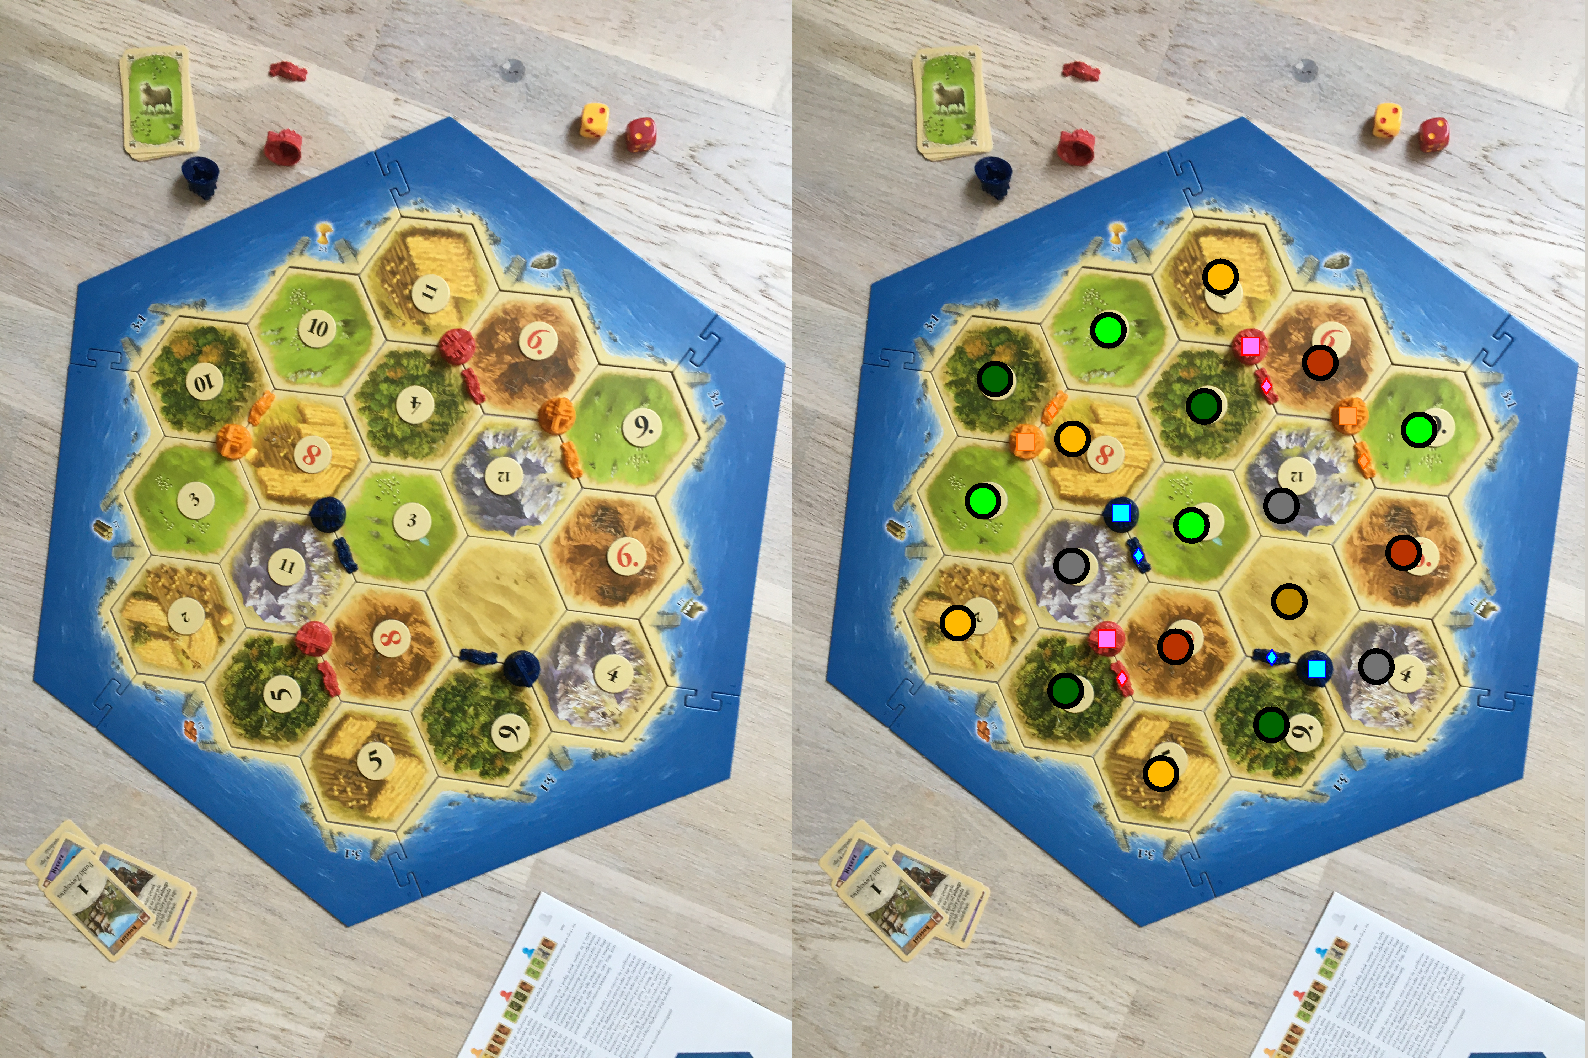
\includegraphics[width=\linewidth]{pictures/results/result21.png}
            \subcaption{Zdjęcie niewyraźne, poruszone}
        \end{subfigure}
        
        
        \begin{subfigure}[]{\linewidth}
            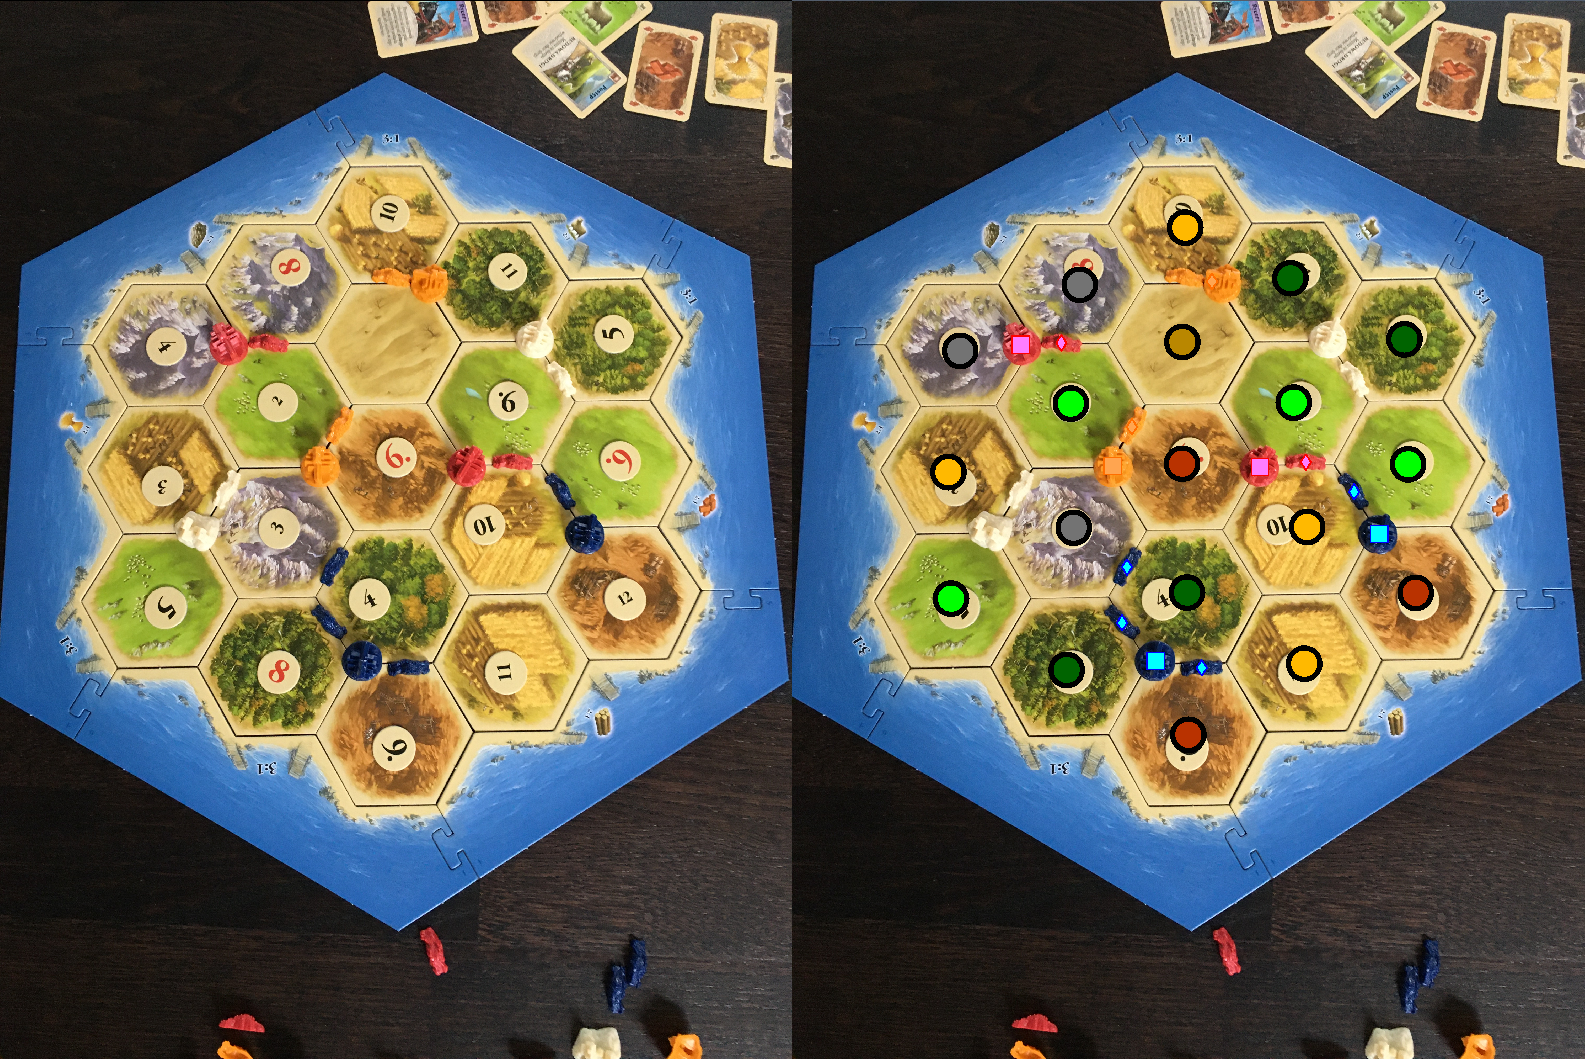
\includegraphics[width=\linewidth]{pictures/results/result11.png}
            \subcaption{Wiele dodatkowych obiektów w tle}
        \end{subfigure}
        
        
        
        \caption{Przykłady zdjęć średnich}
        \label{fig:easy}
    \end{figure}
    
    \subsection{Zdjęcia trudne}
    
    \begin{figure}[H]
        \begin{subfigure}[]{\linewidth}
            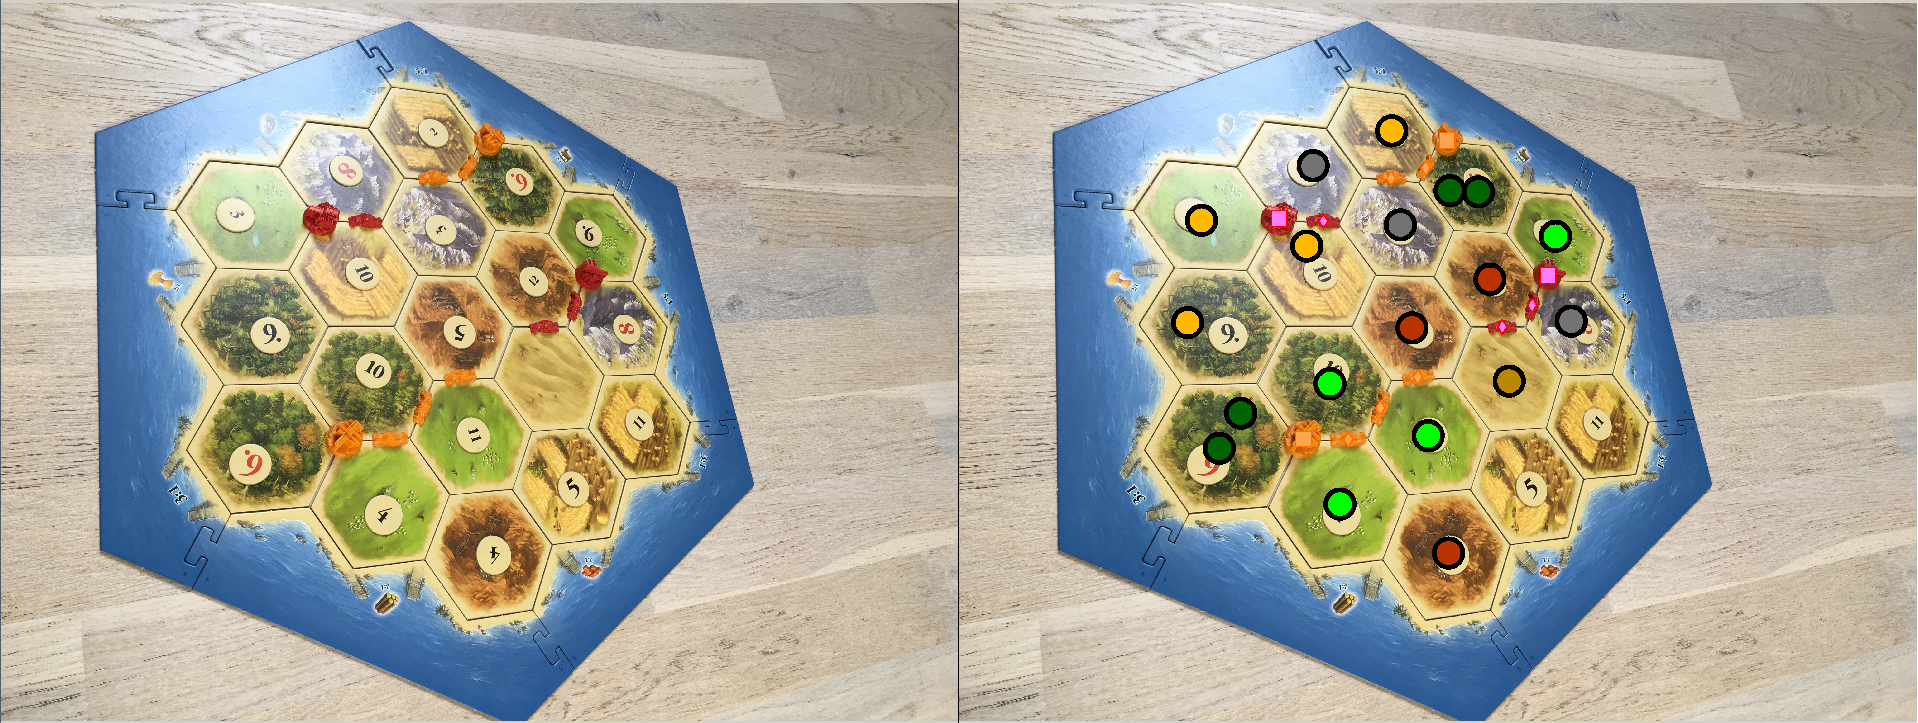
\includegraphics[width=\linewidth]{pictures/hard1.png}
            \subcaption{Rozbłysk na zdjęciu}
        \end{subfigure}
        
        \begin{subfigure}[]{\linewidth}
            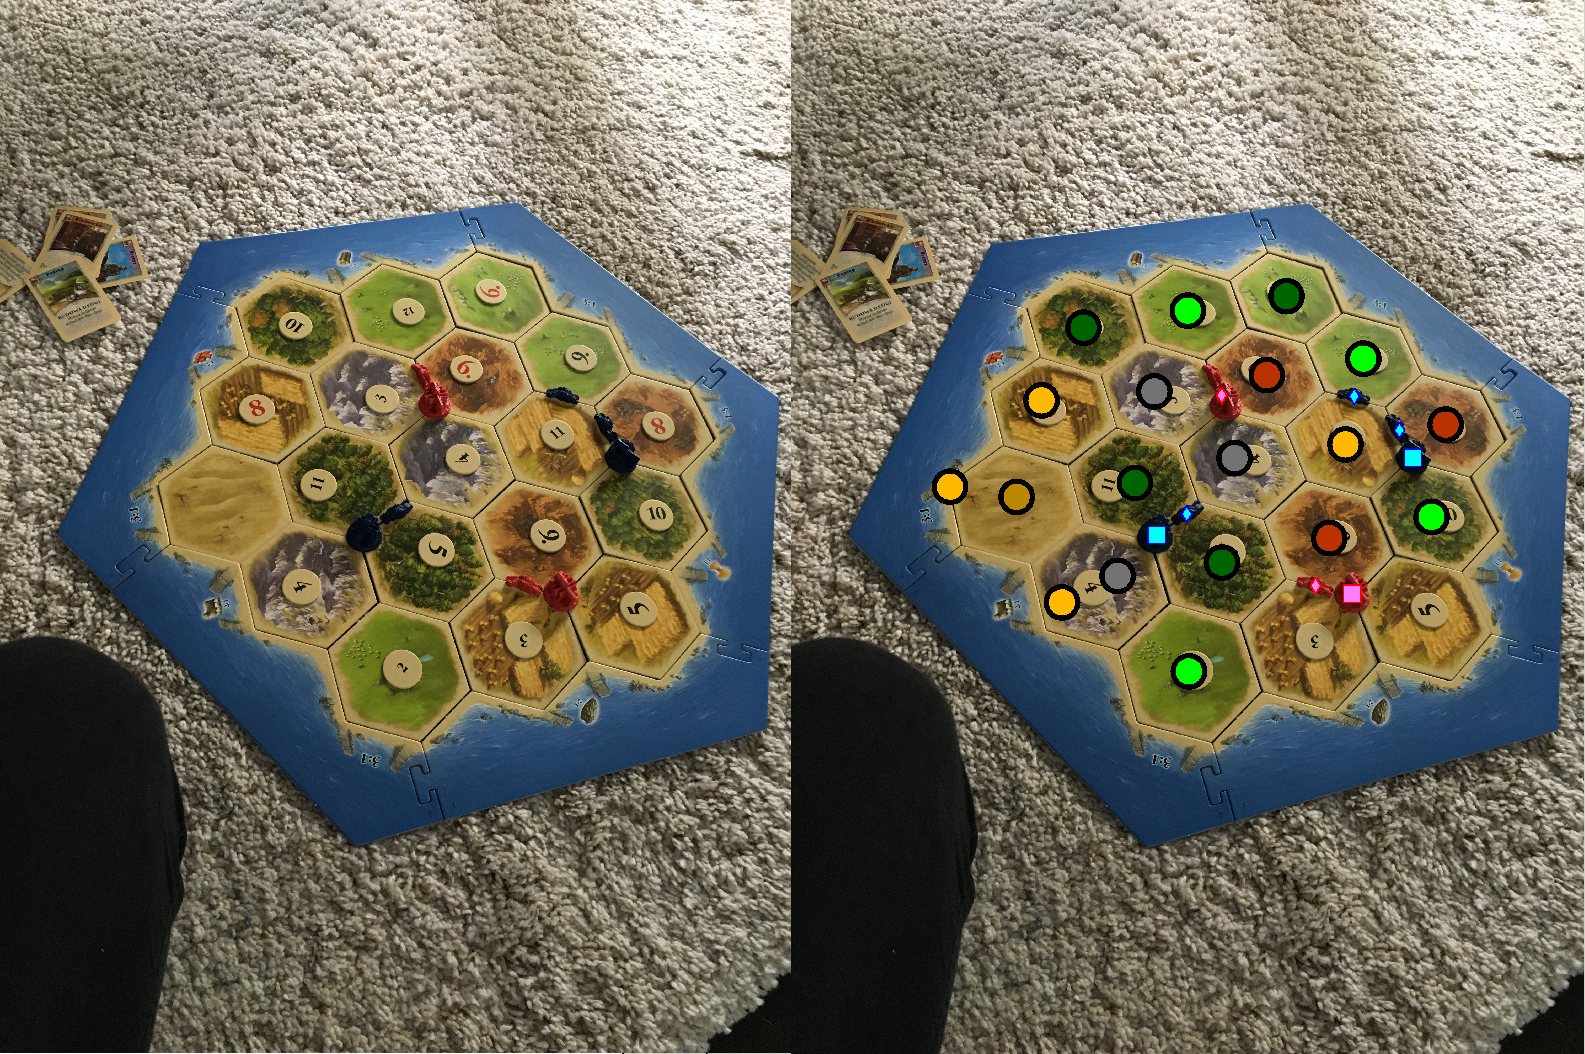
\includegraphics[width=\linewidth]{pictures/results/result03.png}
            \subcaption{Niewystarczająco doświetlone zdjęcie}
        \end{subfigure}

        \caption{Przykłady zdjęć trudnych}
        \label{fig:hard}
    \end{figure}
    
\section{Podsumowanie wyników}
	Program jest w bardzo małym stopniu wrażliwy na obecność dodatkowych elementów na zdjęciu. Krytycznie istotna jest kwestia oświetlenia - mocne rozbłyski, światło pod zbyt ostrym kątem (cienie) oraz nierównomierne i zbyt słabe oświetlenie mogą zaburzyć uzyskiwane wyniki. 
	
	Dodatkowo program opiera się na powtórnych iteracjach algorytmu znajdywania pól, co powoduje, że jeżeli na wczesnym etapie został popełniony błąd, tj. źle zaklasyfikowaliśmy jedno z pól, problem będzie narastał dla kolejnych typów pól. Aby wyeliminować ten problem, należałoby usprawnić metodę wycinania wody, która rozpoznawałaby zaistnienie rozbłysku i uwzględniła go w wycięciu.
	
	 \begin{figure}[H]
        \begin{subfigure}[]{0.5\linewidth}
        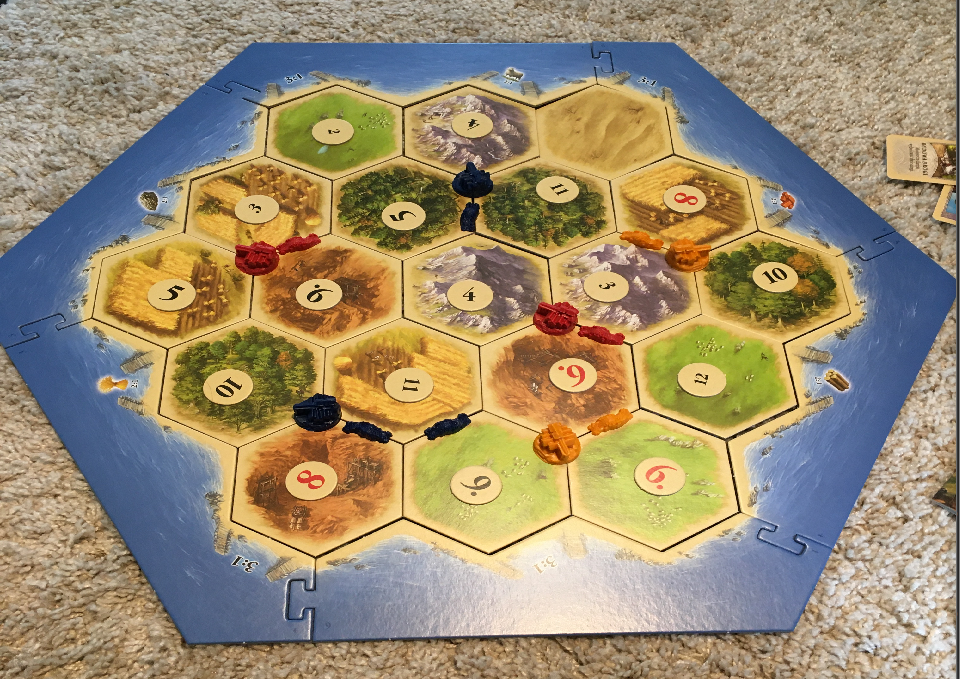
\includegraphics[width=\linewidth]{pictures/fields/flash.png}
        \end{subfigure}
        %
        \begin{subfigure}[]{0.5\linewidth}
        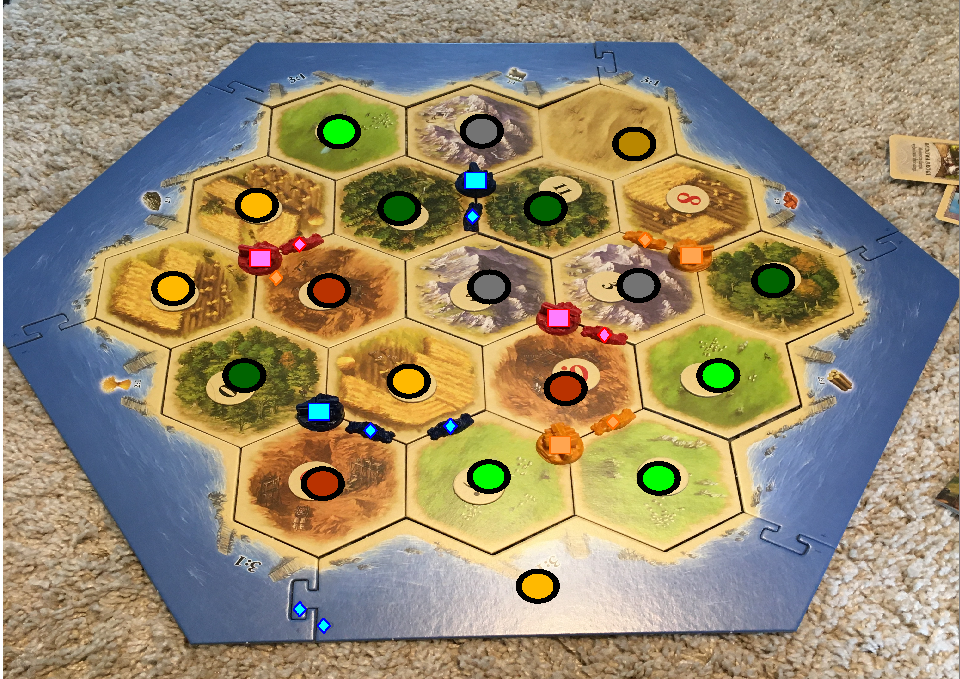
\includegraphics[width=\linewidth]{pictures/fields/after_flash.png}
        \end{subfigure}

        \caption{Rozbłysk na planszy - woda nie zostaje w pełni wycięta, w miejscu rozbłysku
        algorytm znajduje zboże}
        \label{fig:problem_light}
    \end{figure}
    
    Jeżeli oświetlenie jest odpowiednie, program całkiem dobrze radzi sobie ze zdjęciami zrobionymi pod kątem. Trzeba jednak wziąć pod uwagę sytuację, w których pionki z powodu nachylenia zaczynają stawać się jedną całością, bądź zostały źle postawione, tzn. dotykały się. W niektórych przypadkach erozja jest w stanie rozdzielić takie pionki, w innych nie. Aby wyeliminować ten problem, należałoby zaimplementować o wiele bardziej skomplikowany sposób identyfikacji pionków, bazujący nie tylko na ich kształcie i kolorze, ale także na ich ułożeniu względem heksagonów.
		\begin{figure}[H]
        \begin{subfigure}[]{0.5\linewidth}
        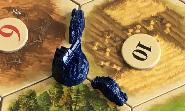
\includegraphics[width=\linewidth]{pictures/fields/angle.png}
        \subcaption{Zbyt duży kąt zdjęcia zlał ze sobą pionki}
        \end{subfigure}
        %
        \begin{subfigure}[]{0.5\linewidth}
        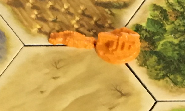
\includegraphics[width=\linewidth]{pictures/fields/touch.png}
        \subcaption{Złe rozstawienie - pionki dotykają się}
        \end{subfigure}

        \caption{Problemy z pionkami}
        \label{fig:problem_pawns}
    \end{figure}

\end{document}
